\documentclass[border=2pt]{standalone}
\usepackage{tikz,amsmath}
\begin{document}
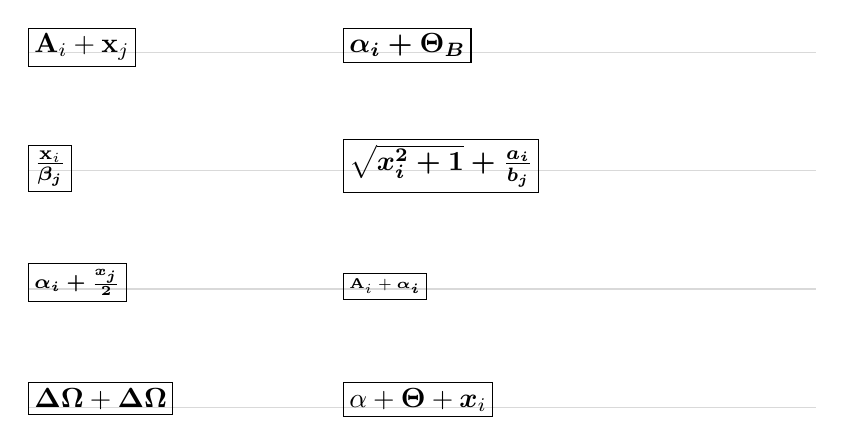
\begin{tikzpicture}
  \draw[gray!30] (0,0)--(10,0) (0,-1.5)--(10,-1.5) (0,-3)--(10,-3) (0,-4.5)--(10,-4.5);
  \node[anchor=base west,draw,inner sep=2pt] at (0,0) {$\mathbf{A}_i+\mathbf{x}_{j}$};
  \node[anchor=base west,draw,inner sep=2pt] at (4,0) {$\boldsymbol{\alpha_i+\Theta_B}$};
  \node[anchor=base west,draw,inner sep=2pt] at (0,-1.5) {$\frac{\mathbf{x}_i}{\boldsymbol{\beta_j}}$};
  \node[anchor=base west,draw,inner sep=2pt,font=\boldmath] at (4,-1.5) {$\sqrt{x_i^2+1}+\frac{a_i}{b_j}$};
  \node[anchor=base west,draw,inner sep=2pt,font=\scriptsize\boldmath] at (0,-3) {$\alpha_i+\frac{x_j}{2}$};
  \node[anchor=base west,draw,inner sep=2pt,font=\tiny] at (4,-3) {$\mathbf{A}_i+\boldsymbol{\alpha_i}$};
  \node[anchor=base west,draw,inner sep=2pt] at (0,-4.5) {$\mathbf{\Delta\Omega}+\boldsymbol{\Delta\Omega}$};
  \node[anchor=base west,draw,inner sep=2pt] at (4,-4.5) {$\mathbf{\alpha+\Theta}+\boldsymbol{x}_i$};
\end{tikzpicture}
\end{document}
